\documentclass[]{book}
\usepackage{lmodern}
\usepackage{amssymb,amsmath}
\usepackage{ifxetex,ifluatex}
\usepackage{fixltx2e} % provides \textsubscript
\ifnum 0\ifxetex 1\fi\ifluatex 1\fi=0 % if pdftex
  \usepackage[T1]{fontenc}
  \usepackage[utf8]{inputenc}
\else % if luatex or xelatex
  \ifxetex
    \usepackage{mathspec}
  \else
    \usepackage{fontspec}
  \fi
  \defaultfontfeatures{Ligatures=TeX,Scale=MatchLowercase}
\fi
% use upquote if available, for straight quotes in verbatim environments
\IfFileExists{upquote.sty}{\usepackage{upquote}}{}
% use microtype if available
\IfFileExists{microtype.sty}{%
\usepackage{microtype}
\UseMicrotypeSet[protrusion]{basicmath} % disable protrusion for tt fonts
}{}
\usepackage{hyperref}
\hypersetup{unicode=true,
            pdftitle={STAT 245 Course Notes},
            pdfauthor={Stacy DeRuiter, Calvin University},
            pdfborder={0 0 0},
            breaklinks=true}
\urlstyle{same}  % don't use monospace font for urls
\usepackage{natbib}
\bibliographystyle{apalike}
\usepackage{color}
\usepackage{fancyvrb}
\newcommand{\VerbBar}{|}
\newcommand{\VERB}{\Verb[commandchars=\\\{\}]}
\DefineVerbatimEnvironment{Highlighting}{Verbatim}{commandchars=\\\{\}}
% Add ',fontsize=\small' for more characters per line
\usepackage{framed}
\definecolor{shadecolor}{RGB}{248,248,248}
\newenvironment{Shaded}{\begin{snugshade}}{\end{snugshade}}
\newcommand{\AlertTok}[1]{\textcolor[rgb]{0.94,0.16,0.16}{#1}}
\newcommand{\AnnotationTok}[1]{\textcolor[rgb]{0.56,0.35,0.01}{\textbf{\textit{#1}}}}
\newcommand{\AttributeTok}[1]{\textcolor[rgb]{0.77,0.63,0.00}{#1}}
\newcommand{\BaseNTok}[1]{\textcolor[rgb]{0.00,0.00,0.81}{#1}}
\newcommand{\BuiltInTok}[1]{#1}
\newcommand{\CharTok}[1]{\textcolor[rgb]{0.31,0.60,0.02}{#1}}
\newcommand{\CommentTok}[1]{\textcolor[rgb]{0.56,0.35,0.01}{\textit{#1}}}
\newcommand{\CommentVarTok}[1]{\textcolor[rgb]{0.56,0.35,0.01}{\textbf{\textit{#1}}}}
\newcommand{\ConstantTok}[1]{\textcolor[rgb]{0.00,0.00,0.00}{#1}}
\newcommand{\ControlFlowTok}[1]{\textcolor[rgb]{0.13,0.29,0.53}{\textbf{#1}}}
\newcommand{\DataTypeTok}[1]{\textcolor[rgb]{0.13,0.29,0.53}{#1}}
\newcommand{\DecValTok}[1]{\textcolor[rgb]{0.00,0.00,0.81}{#1}}
\newcommand{\DocumentationTok}[1]{\textcolor[rgb]{0.56,0.35,0.01}{\textbf{\textit{#1}}}}
\newcommand{\ErrorTok}[1]{\textcolor[rgb]{0.64,0.00,0.00}{\textbf{#1}}}
\newcommand{\ExtensionTok}[1]{#1}
\newcommand{\FloatTok}[1]{\textcolor[rgb]{0.00,0.00,0.81}{#1}}
\newcommand{\FunctionTok}[1]{\textcolor[rgb]{0.00,0.00,0.00}{#1}}
\newcommand{\ImportTok}[1]{#1}
\newcommand{\InformationTok}[1]{\textcolor[rgb]{0.56,0.35,0.01}{\textbf{\textit{#1}}}}
\newcommand{\KeywordTok}[1]{\textcolor[rgb]{0.13,0.29,0.53}{\textbf{#1}}}
\newcommand{\NormalTok}[1]{#1}
\newcommand{\OperatorTok}[1]{\textcolor[rgb]{0.81,0.36,0.00}{\textbf{#1}}}
\newcommand{\OtherTok}[1]{\textcolor[rgb]{0.56,0.35,0.01}{#1}}
\newcommand{\PreprocessorTok}[1]{\textcolor[rgb]{0.56,0.35,0.01}{\textit{#1}}}
\newcommand{\RegionMarkerTok}[1]{#1}
\newcommand{\SpecialCharTok}[1]{\textcolor[rgb]{0.00,0.00,0.00}{#1}}
\newcommand{\SpecialStringTok}[1]{\textcolor[rgb]{0.31,0.60,0.02}{#1}}
\newcommand{\StringTok}[1]{\textcolor[rgb]{0.31,0.60,0.02}{#1}}
\newcommand{\VariableTok}[1]{\textcolor[rgb]{0.00,0.00,0.00}{#1}}
\newcommand{\VerbatimStringTok}[1]{\textcolor[rgb]{0.31,0.60,0.02}{#1}}
\newcommand{\WarningTok}[1]{\textcolor[rgb]{0.56,0.35,0.01}{\textbf{\textit{#1}}}}
\usepackage{longtable,booktabs}
\usepackage{graphicx,grffile}
\makeatletter
\def\maxwidth{\ifdim\Gin@nat@width>\linewidth\linewidth\else\Gin@nat@width\fi}
\def\maxheight{\ifdim\Gin@nat@height>\textheight\textheight\else\Gin@nat@height\fi}
\makeatother
% Scale images if necessary, so that they will not overflow the page
% margins by default, and it is still possible to overwrite the defaults
% using explicit options in \includegraphics[width, height, ...]{}
\setkeys{Gin}{width=\maxwidth,height=\maxheight,keepaspectratio}
\IfFileExists{parskip.sty}{%
\usepackage{parskip}
}{% else
\setlength{\parindent}{0pt}
\setlength{\parskip}{6pt plus 2pt minus 1pt}
}
\setlength{\emergencystretch}{3em}  % prevent overfull lines
\providecommand{\tightlist}{%
  \setlength{\itemsep}{0pt}\setlength{\parskip}{0pt}}
\setcounter{secnumdepth}{5}
% Redefines (sub)paragraphs to behave more like sections
\ifx\paragraph\undefined\else
\let\oldparagraph\paragraph
\renewcommand{\paragraph}[1]{\oldparagraph{#1}\mbox{}}
\fi
\ifx\subparagraph\undefined\else
\let\oldsubparagraph\subparagraph
\renewcommand{\subparagraph}[1]{\oldsubparagraph{#1}\mbox{}}
\fi

%%% Use protect on footnotes to avoid problems with footnotes in titles
\let\rmarkdownfootnote\footnote%
\def\footnote{\protect\rmarkdownfootnote}

%%% Change title format to be more compact
\usepackage{titling}

% Create subtitle command for use in maketitle
\providecommand{\subtitle}[1]{
  \posttitle{
    \begin{center}\large#1\end{center}
    }
}

\setlength{\droptitle}{-2em}

  \title{STAT 245 Course Notes}
    \pretitle{\vspace{\droptitle}\centering\huge}
  \posttitle{\par}
    \author{Stacy DeRuiter, Calvin University}
    \preauthor{\centering\large\emph}
  \postauthor{\par}
      \predate{\centering\large\emph}
  \postdate{\par}
    \date{2019-09-26}

\usepackage{booktabs}
\usepackage{amsthm}
\makeatletter
\def\thm@space@setup{%
  \thm@preskip=8pt plus 2pt minus 4pt
  \thm@postskip=\thm@preskip
}
\makeatother

\begin{document}
\maketitle

{
\setcounter{tocdepth}{1}
\tableofcontents
}
\hypertarget{description}{%
\chapter{Description}\label{description}}

This is a set of course notes distributed in STAT 245 at Calvin University in Fall 2019. Contact sld33 at calvin.edu with comments, corrections or suggestions.

\hypertarget{linear-regression}{%
\chapter{Linear Regression}\label{linear-regression}}

You probably learned something about linear regression in a previous course. Here, we briefly review the main concepts of simple linear regression and quickly expand our tool box to multiple regression (with both quantitative and categorical predictors).

\hypertarget{data}{%
\section{Data}\label{data}}

We will consider a small dataset from an article by J.S. Martin and colleagues, titled \href{https://royalsocietypublishing.org/doi/suppl/10.1098/rsbl.2019.0232}{\emph{Facial width-to-height ratio is associated with agonistic and affiliative dominance in bonobos (\textbf{Pan paniscus})}}

Notes: variable \texttt{fWHR} is the facial width-height ratio and \texttt{AssR} is the Assertiveness score of affiliative dominance. \texttt{normDS} is another dominance score. A few figures of the data are below - we will do some more exploration together.

\begin{verbatim}
## Observations: 117
## Variables: 8
## $ Name   <fct> Zuani, Zuani, Zorba, Zorba, Zorba, Zomi, Zomi, Zamba, Z...
## $ Group  <fct> Apenheul, Apenheul, Wilhelma, Wilhelma, Wilhelma, Frank...
## $ Sex    <fct> Female, Female, Male, Male, Male, Female, Female, Male,...
## $ Age    <int> 22, 22, 34, 34, 34, 15, 15, 14, 14, 14, 18, 18, 18, 18,...
## $ fWHR   <dbl> 1.475052, 1.321814, 1.581446, 1.479237, 1.390086, 1.340...
## $ AssR   <dbl> 5.36, 5.36, 2.36, 2.36, 2.36, 3.92, 3.92, 4.74, 4.74, 4...
## $ normDS <dbl> 1.430, 1.430, 2.341, 2.341, 2.341, 3.087, 3.087, 3.035,...
## $ weight <dbl> 24.0, 24.0, NA, NA, NA, NA, NA, 41.6, 41.6, 41.6, 38.0,...
\end{verbatim}

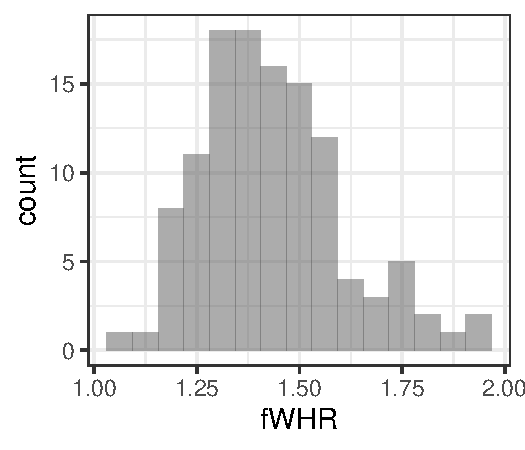
\includegraphics{bookdown-demo_files/figure-latex/view-data-1.pdf} 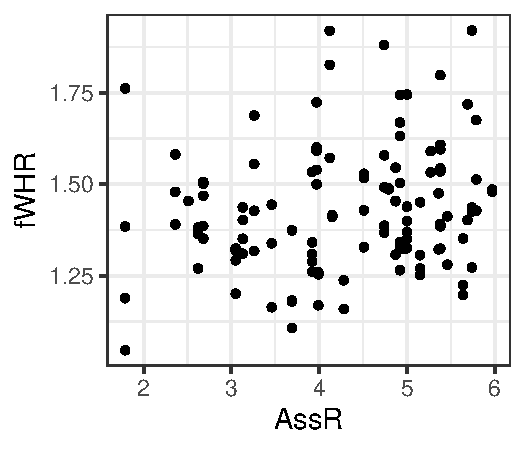
\includegraphics{bookdown-demo_files/figure-latex/view-data-2.pdf}

\hypertarget{simple-linear-regression-residuals-least-squares}{%
\section{Simple linear regression, Residuals \& Least squares}\label{simple-linear-regression-residuals-least-squares}}

First, let's review and consider a simple (one-predictor) linear regression model. Fit the model

\begin{Shaded}
\begin{Highlighting}[]
\NormalTok{slr <-}\StringTok{ }\KeywordTok{lm}\NormalTok{(fWHR }\OperatorTok{~}\StringTok{ }\NormalTok{AssR, }\DataTypeTok{data=}\NormalTok{bonobos)}
\end{Highlighting}
\end{Shaded}

Extract the slope and intercept values:

\begin{Shaded}
\begin{Highlighting}[]
\KeywordTok{coef}\NormalTok{(slr)}
\end{Highlighting}
\end{Shaded}

\begin{verbatim}
## (Intercept)        AssR 
##  1.30685287  0.02918242
\end{verbatim}

Add the regression line to the plot:

\begin{Shaded}
\begin{Highlighting}[]
\KeywordTok{gf_point}\NormalTok{(fWHR }\OperatorTok{~}\StringTok{ }\NormalTok{AssR, }\DataTypeTok{data=}\NormalTok{bonobos) }\OperatorTok\StringTok{ }
\StringTok{  }\KeywordTok{gf_lm}\NormalTok{()}
\end{Highlighting}
\end{Shaded}

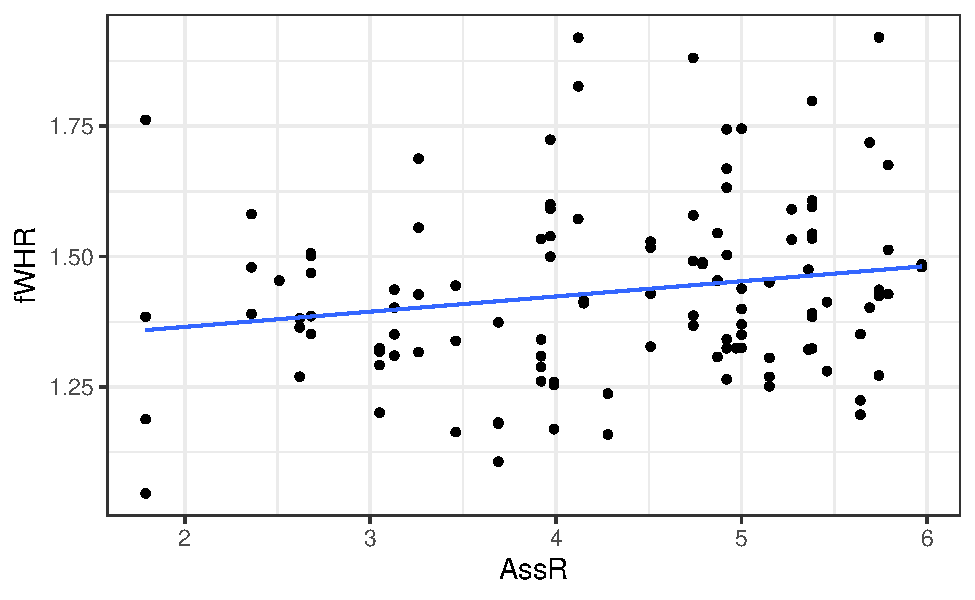
\includegraphics{bookdown-demo_files/figure-latex/lm-scatter-with-line-1.pdf}

\begin{Shaded}
\begin{Highlighting}[]
\KeywordTok{summary}\NormalTok{(slr)}
\end{Highlighting}
\end{Shaded}

\begin{verbatim}
## 
## Call:
## lm(formula = fWHR ~ AssR, data = bonobos)
## 
## Residuals:
##      Min       1Q   Median       3Q      Max 
## -0.31320 -0.11369 -0.01242  0.09008  0.49241 
## 
## Coefficients:
##             Estimate Std. Error t value Pr(>|t|)    
## (Intercept)  1.30685    0.06283  20.801   <2e-16 ***
## AssR         0.02918    0.01420   2.055   0.0421 *  
## ---
## Signif. codes:  0 '***' 0.001 '**' 0.01 '*' 0.05 '.' 0.1 ' ' 1
## 
## Residual standard error: 0.1689 on 115 degrees of freedom
## Multiple R-squared:  0.03542,    Adjusted R-squared:  0.02704 
## F-statistic: 4.223 on 1 and 115 DF,  p-value: 0.04213
\end{verbatim}

\hypertarget{using-lm-to-fit-a-linear-regression-in-r}{%
\subsection{\texorpdfstring{Using \texttt{lm()} to fit a linear regression in R}{Using lm() to fit a linear regression in R}}\label{using-lm-to-fit-a-linear-regression-in-r}}

\hypertarget{equation-of-the-fitted-regression-line}{%
\subsection{Equation of the fitted regression line}\label{equation-of-the-fitted-regression-line}}

\hypertarget{multiple-regression}{%
\section{Multiple regression}\label{multiple-regression}}

Rarely does our response variable \textbf{really} depend on only one predictor. Can we improve the model by adding more predictors?

\begin{Shaded}
\begin{Highlighting}[]
\NormalTok{mlr <-}\StringTok{ }\KeywordTok{lm}\NormalTok{(fWHR }\OperatorTok{~}\StringTok{ }\NormalTok{AssR }\OperatorTok{+}\StringTok{ }\NormalTok{weight, }\DataTypeTok{data=}\NormalTok{bonobos)}
\KeywordTok{coef}\NormalTok{(mlr)}
\end{Highlighting}
\end{Shaded}

\begin{verbatim}
## (Intercept)        AssR      weight 
## 0.944790930 0.039888045 0.008644299
\end{verbatim}

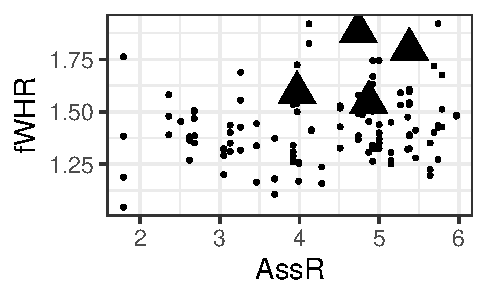
\includegraphics{bookdown-demo_files/figure-latex/mult-reg-plots-1.pdf} 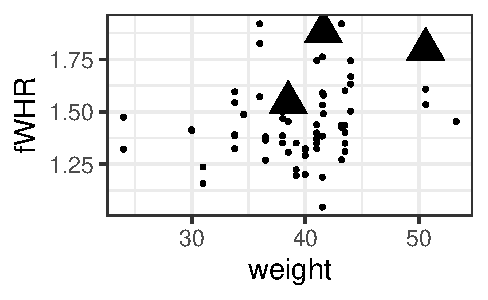
\includegraphics{bookdown-demo_files/figure-latex/mult-reg-plots-2.pdf}

\hypertarget{is-it-really-better}{%
\subsection{Is it really better?}\label{is-it-really-better}}

How do we know if the model with more predictors is ``better''? (For a more detailed answer, wait about a week\ldots) But before we can define a ``beter'' model: how did R find the ``best'' intercept and slopes?

\hypertarget{regression-residuals-errors}{%
\subsection{Regression residuals = ``errors''}\label{regression-residuals-errors}}

\hypertarget{computing-predictions}{%
\subsection{Computing Predictions}\label{computing-predictions}}

Use the regression equation to compute \textbf{predicted values} for the three data points below:

\begin{verbatim}
##        fWHR AssR weight
## 8  1.880866 4.74   41.6
## 25 1.798387 5.38   50.6
## 41 1.591440 3.97     NA
## 65 1.545019 4.87   38.5
\end{verbatim}

\hypertarget{predictors-with-two-categories}{%
\section{Predictors with two categories}\label{predictors-with-two-categories}}

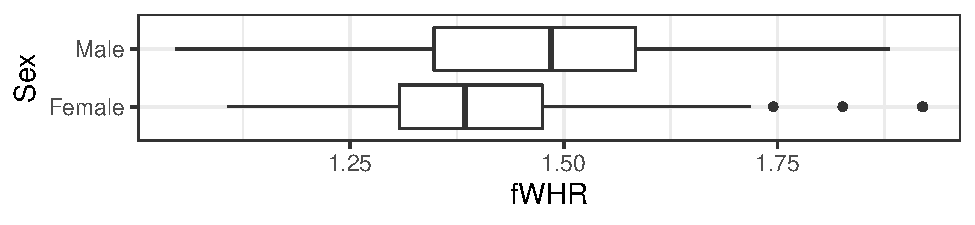
\includegraphics{bookdown-demo_files/figure-latex/unnamed-chunk-2-1.pdf}

\begin{Shaded}
\begin{Highlighting}[]
\NormalTok{mlr2 <-}\StringTok{ }\KeywordTok{lm}\NormalTok{(fWHR }\OperatorTok{~}\StringTok{ }\NormalTok{AssR }\OperatorTok{+}\StringTok{ }\NormalTok{weight }\OperatorTok{+}\StringTok{ }\NormalTok{Sex, }\DataTypeTok{data =}\NormalTok{ bonobos)}
\KeywordTok{coef}\NormalTok{(mlr2)}
\end{Highlighting}
\end{Shaded}

\begin{verbatim}
## (Intercept)        AssR      weight     SexMale 
## 1.065420976 0.058435841 0.002257142 0.128484275
\end{verbatim}

How does the model incorporate this covariate mathematically?

\hypertarget{predictors-with-more-categories}{%
\subsection{Predictors with more categories}\label{predictors-with-more-categories}}

\begin{Shaded}
\begin{Highlighting}[]
\KeywordTok{gf_boxplot}\NormalTok{(fWHR }\OperatorTok{~}\StringTok{ }\NormalTok{Group, }\DataTypeTok{data =}\NormalTok{ bonobos)}
\end{Highlighting}
\end{Shaded}

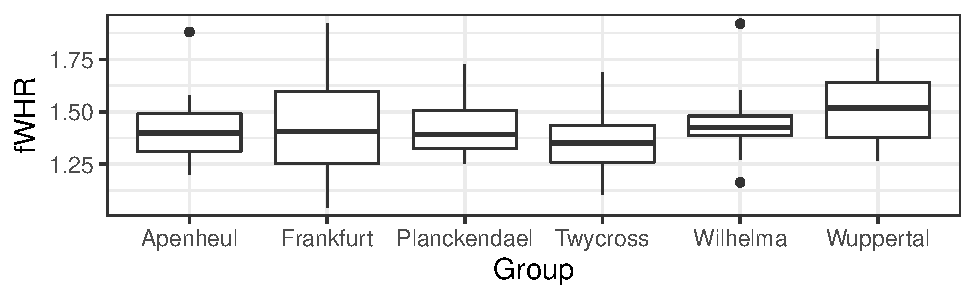
\includegraphics{bookdown-demo_files/figure-latex/unnamed-chunk-4-1.pdf}

\begin{Shaded}
\begin{Highlighting}[]
\NormalTok{mlr3 <-}\StringTok{ }\KeywordTok{lm}\NormalTok{(fWHR }\OperatorTok{~}\StringTok{ }\NormalTok{AssR }\OperatorTok{+}\StringTok{ }\NormalTok{weight }\OperatorTok{+}\StringTok{ }\NormalTok{Sex }\OperatorTok{+}\StringTok{ }\NormalTok{Group, }\DataTypeTok{data =}\NormalTok{ bonobos)}
\KeywordTok{coef}\NormalTok{(mlr3)}
\end{Highlighting}
\end{Shaded}

\begin{verbatim}
##       (Intercept)              AssR            weight           SexMale 
##       1.007734691       0.064361973       0.003458979       0.124854271 
##    GroupFrankfurt GroupPlanckendael     GroupTwycross     GroupWilhelma 
##       0.037426358      -0.008464572      -0.112907589       0.011186724 
##    GroupWuppertal 
##      -0.004364826
\end{verbatim}

How does the model incorporate \textbf{this} covariate mathematically?

\hypertarget{returning-to-the-r-model-summary}{%
\section{Returning to the R Model Summary}\label{returning-to-the-r-model-summary}}

There are several bits of information you should be able to extract from the \texttt{summary()} output R produces on a fitted linear regression model:

\begin{itemize}
\item
  \(\beta\)s, Coefficient Estimates
\item
  \(\sigma\), labeled ``residual standard error''
\item
  \(R^2\) (adjusted)
\end{itemize}

\begin{Shaded}
\begin{Highlighting}[]
\NormalTok{mlr3 <-}\StringTok{ }\KeywordTok{lm}\NormalTok{(fWHR }\OperatorTok{~}\StringTok{ }\NormalTok{AssR }\OperatorTok{+}\StringTok{ }\NormalTok{weight }\OperatorTok{+}\StringTok{ }\NormalTok{Sex }\OperatorTok{+}\StringTok{ }\NormalTok{Group, }\DataTypeTok{data =}\NormalTok{ bonobos)}
\KeywordTok{summary}\NormalTok{(mlr3)}
\end{Highlighting}
\end{Shaded}

\begin{verbatim}
## 
## Call:
## lm(formula = fWHR ~ AssR + weight + Sex + Group, data = bonobos)
## 
## Residuals:
##      Min       1Q   Median       3Q      Max 
## -0.38288 -0.09488 -0.02642  0.07196  0.48464 
## 
## Coefficients:
##                    Estimate Std. Error t value Pr(>|t|)    
## (Intercept)        1.007735   0.217585   4.631 2.05e-05 ***
## AssR               0.064362   0.021158   3.042   0.0035 ** 
## weight             0.003459   0.005547   0.624   0.5353    
## SexMale            0.124854   0.059278   2.106   0.0394 *  
## GroupFrankfurt     0.037426   0.074892   0.500   0.6191    
## GroupPlanckendael -0.008465   0.075407  -0.112   0.9110    
## GroupTwycross     -0.112908   0.074779  -1.510   0.1364    
## GroupWilhelma      0.011187   0.085538   0.131   0.8964    
## GroupWuppertal    -0.004365   0.071292  -0.061   0.9514    
## ---
## Signif. codes:  0 '***' 0.001 '**' 0.01 '*' 0.05 '.' 0.1 ' ' 1
## 
## Residual standard error: 0.1691 on 59 degrees of freedom
##   (49 observations deleted due to missingness)
## Multiple R-squared:  0.2517, Adjusted R-squared:  0.1502 
## F-statistic:  2.48 on 8 and 59 DF,  p-value: 0.02167
\end{verbatim}

\hypertarget{predictions-from-the-model}{%
\section{Predictions from the model}\label{predictions-from-the-model}}

\hypertarget{by-hand}{%
\subsection{By Hand}\label{by-hand}}

The equation for the fitted model above is:

\[ y = \beta_0 + \beta_1x_1 + \beta_2x_2 + \beta_3I_{Male} + \beta_4I_{Frankfurt} + \beta_5I_{Planckendael} + \beta_6I_{Twycross} + \beta_7I_{Wilhelma} + \beta_7I_{Wuppertal} + \epsilon\]

where

\begin{itemize}
\tightlist
\item
  \(y =\)
\item
  \(\beta_0=\)
\end{itemize}

\begin{itemize}
\tightlist
\item
  \(x_1=\)
\item
  \(x_2=\)
\item
  \(\beta_1, \beta_2, \beta_3 ...\) are:
\item
  \(I_{Male} =\)
\item
  \(I_{Frankfurt} =\)
\item
  \(I_{Planckendael} =\) \hspace{3in}, etc.
\item
  \(\epsilon=\)
\end{itemize}

\hypertarget{comprehension-check}{%
\subsubsection{Comprehension check:}\label{comprehension-check}}

What is the expected fWHR (according to this model) for a 30 kg female bonobo at the Wilhelma zoo?

\hypertarget{prediction-plots-in-r}{%
\subsection{Prediction Plots in R}\label{prediction-plots-in-r}}

We can ask R to compute predictions for \textbf{all} the data points in the real dataset.

\begin{Shaded}
\begin{Highlighting}[]
\NormalTok{bonobos <-}\StringTok{ }\NormalTok{bonobos }\OperatorTok\StringTok{ }
\StringTok{  }\KeywordTok{mutate}\NormalTok{(}\DataTypeTok{preds =} \KeywordTok{predict}\NormalTok{(mlr3))}
\end{Highlighting}
\end{Shaded}

\begin{verbatim}
## Error: Column `preds` must be length 117 (the number of rows) or one, not 68
\end{verbatim}

Wait, what? This error is because the \texttt{lm()} function removes rows containing missing values from the dataset, so it computes only 68 residuals (for the complete cases in the data). This doesn't match the 117 rows in the original data. We can solve the problem by omitting rows with missing values first. To be safe, we first select only the variables we need, so we don't omit rows based on missing values in unused variables.

\begin{Shaded}
\begin{Highlighting}[]
\NormalTok{b2 <-}\StringTok{ }\NormalTok{bonobos }\OperatorTok
\StringTok{  }\KeywordTok{select}\NormalTok{(fWHR, weight, AssR, Sex, Group) }\OperatorTok
\StringTok{  }\KeywordTok{na.omit}\NormalTok{() }\OperatorTok
\StringTok{  }\KeywordTok{mutate}\NormalTok{(}\DataTypeTok{preds =} \KeywordTok{predict}\NormalTok{(mlr3))}
\end{Highlighting}
\end{Shaded}

\emph{We have a full set of predictions!}

But if we plot these predictions on a scatter plot of \texttt{fWHR} as a function of \texttt{AssR}, we \emph{do not} get a straight line, because the predictions are also impacted by varying values of \texttt{weight}, \texttt{Sex}, and \texttt{Group}:

\begin{Shaded}
\begin{Highlighting}[]
\KeywordTok{gf_point}\NormalTok{(fWHR }\OperatorTok{~}\StringTok{ }\NormalTok{AssR, }\DataTypeTok{data =}\NormalTok{ b2) }\OperatorTok
\StringTok{  }\KeywordTok{gf_line}\NormalTok{(preds }\OperatorTok{~}\StringTok{ }\NormalTok{AssR, }\DataTypeTok{data=}\NormalTok{b2)}
\end{Highlighting}
\end{Shaded}

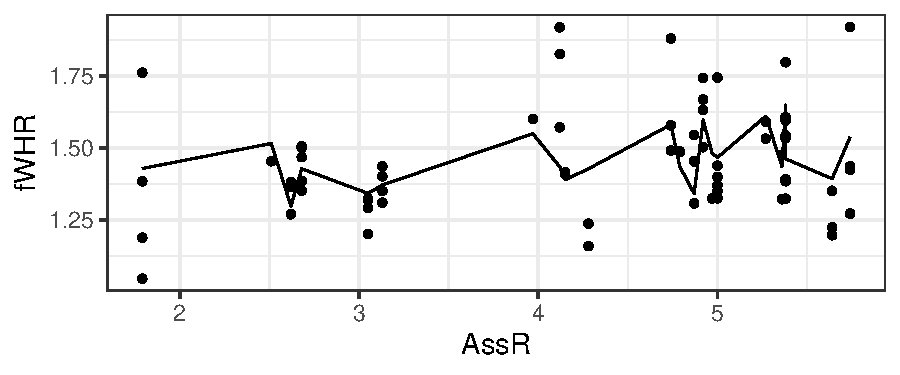
\includegraphics{bookdown-demo_files/figure-latex/unnamed-chunk-8-1.pdf}

\emph{But\ldots we would really like a straight line that helps us visualize the meaning of the \(\beta\) (slope coefficient) for \texttt{AssR}.} We can make predictions for a \textbf{hypothetical} dataset, in which \texttt{AssR} varies over a reasonable range, but the other predictors stay constant. This lets us see how \texttt{AssR} (and only \texttt{AssR}) affects the response, without contributions from other predictors. In choosing the values to include in hypothetical dataset, we often choose to hold variables constant at their most common or median values, but not blindly: also, avoid impossible or implausible variable combinations (for example, specifying that a person lives in the state of Michigan but the city of Chicago, or that they are a 5-year-old person with 4 children). \emph{In this case, to match the figures in the published paper, we are also going to vary the \texttt{Sex} - but generally you'd only allow one predictor to vary.}

\begin{Shaded}
\begin{Highlighting}[]
\NormalTok{fake_data <-}\StringTok{ }\KeywordTok{expand.grid}\NormalTok{(}\DataTypeTok{AssR =} \KeywordTok{seq}\NormalTok{(}\DataTypeTok{from=}\FloatTok{1.8}\NormalTok{, }\DataTypeTok{to=}\FloatTok{5.7}\NormalTok{, }\DataTypeTok{by=}\FloatTok{0.05}\NormalTok{),}
                         \DataTypeTok{weight =} \FloatTok{38.5}\NormalTok{,}
                         \DataTypeTok{Sex =} \KeywordTok{c}\NormalTok{(}\StringTok{'Female'}\NormalTok{, }\StringTok{'Male'}\NormalTok{),}
                         \DataTypeTok{Group =} \StringTok{'Wuppertal'}\NormalTok{)}

\NormalTok{fake_data <-}\StringTok{ }\NormalTok{fake_data }\OperatorTok\StringTok{ }
\StringTok{  }\KeywordTok{mutate}\NormalTok{(}\DataTypeTok{preds =} \KeywordTok{predict}\NormalTok{(mlr3, }\DataTypeTok{newdata =}\NormalTok{ fake_data))}
\KeywordTok{gf_line}\NormalTok{(preds }\OperatorTok{~}\StringTok{ }\NormalTok{AssR, }\DataTypeTok{color =} \OperatorTok{~}\NormalTok{Sex, }\DataTypeTok{data=}\NormalTok{fake_data) }\OperatorTok\StringTok{ }\KeywordTok{gf_labs}\NormalTok{(}\DataTypeTok{y=}\StringTok{'Predicted}\CharTok{\textbackslash{}n}\StringTok{fWHR'}\NormalTok{)}
\end{Highlighting}
\end{Shaded}

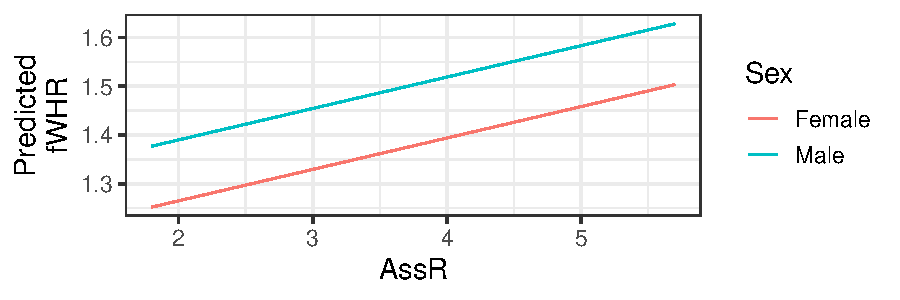
\includegraphics{bookdown-demo_files/figure-latex/unnamed-chunk-9-1.pdf}

\hypertarget{comprehension-checks}{%
\subsubsection{Comprehension checks:}\label{comprehension-checks}}

\begin{itemize}
\tightlist
\item
  Should we overlay prediction-plot line(s) on the data scatter plot?
\item
  How do you think the plot would look if we changed the constant predictor values?
\item
  What is missing from this picture?
\end{itemize}

\hypertarget{shortcut}{%
\subsubsection{Shortcut}\label{shortcut}}

\begin{Shaded}
\begin{Highlighting}[]
\KeywordTok{require}\NormalTok{(s245)}
\KeywordTok{pred_plot}\NormalTok{(mlr3, }\StringTok{'AssR'}\NormalTok{)}
\end{Highlighting}
\end{Shaded}

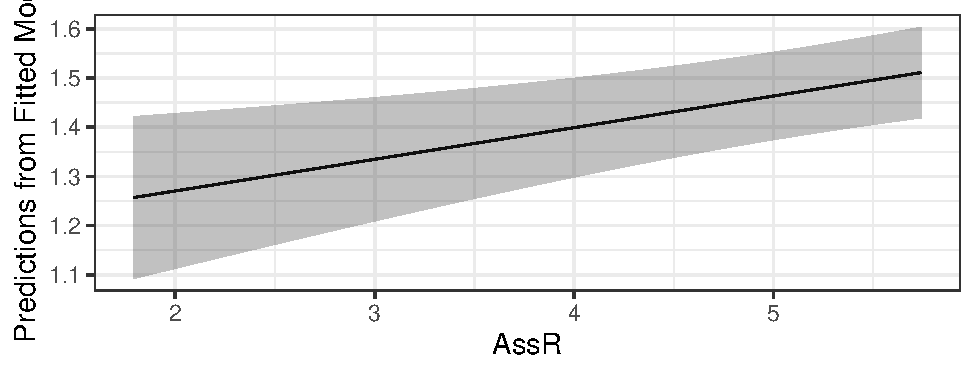
\includegraphics{bookdown-demo_files/figure-latex/unnamed-chunk-10-1.pdf}

\hypertarget{why-are-we-doing-this-again}{%
\section{Why are we doing this again?}\label{why-are-we-doing-this-again}}

Why make prediction plots?

\hypertarget{shortcut-method---with-uncertainty}{%
\section{Shortcut Method - With Uncertainty}\label{shortcut-method---with-uncertainty}}

We saw before that \texttt{pred\_plot()} makes it very easy for us to generate prediction plots showing what a (multiple regression) model says about the relationship between the response and \emph{one} of the predictors:

\begin{Shaded}
\begin{Highlighting}[]
\KeywordTok{require}\NormalTok{(s245)}
\KeywordTok{pred_plot}\NormalTok{(mlr3, }\StringTok{'AssR'}\NormalTok{) }\OperatorTok
\StringTok{  }\KeywordTok{gf_labs}\NormalTok{(}\DataTypeTok{y =} \StringTok{'Predicted fWHR'}\NormalTok{)}
\end{Highlighting}
\end{Shaded}

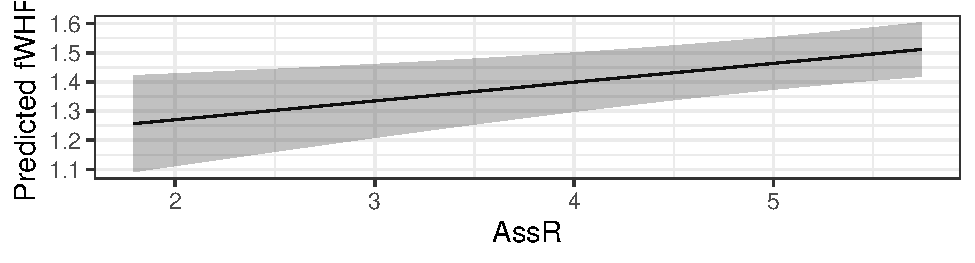
\includegraphics{bookdown-demo_files/figure-latex/unnamed-chunk-11-1.pdf}

\emph{Note the custom axis label - otherwise you get a long, unwieldy default ``Predictions from fitted model''}

\begin{Shaded}
\begin{Highlighting}[]
\KeywordTok{require}\NormalTok{(s245)}
\KeywordTok{pred_plot}\NormalTok{(mlr3, }\StringTok{'Group'}\NormalTok{) }\OperatorTok
\StringTok{  }\KeywordTok{gf_labs}\NormalTok{(}\DataTypeTok{y =} \StringTok{'Predicted fWHR'}\NormalTok{)}
\end{Highlighting}
\end{Shaded}

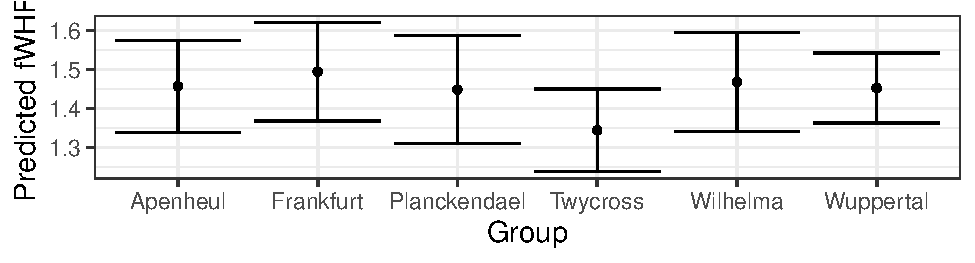
\includegraphics{bookdown-demo_files/figure-latex/unnamed-chunk-12-1.pdf}

They look nice! But they should raise two questions:

\begin{itemize}
\item
  Uncertainty:
\item
  Fixed values:
\end{itemize}

\begin{Shaded}
\begin{Highlighting}[]
\KeywordTok{get_fixed}\NormalTok{(bonobos)  }\OperatorTok\StringTok{ }
\StringTok{  }\NormalTok{pander}\OperatorTok{::}\KeywordTok{pander}\NormalTok{()}
\end{Highlighting}
\end{Shaded}

\begin{longtable}[]{@{}cccccccccc@{}}
\toprule
\begin{minipage}[b]{0.06\columnwidth}\centering
Name\strut
\end{minipage} & \begin{minipage}[b]{0.10\columnwidth}\centering
Group\strut
\end{minipage} & \begin{minipage}[b]{0.08\columnwidth}\centering
Sex\strut
\end{minipage} & \begin{minipage}[b]{0.05\columnwidth}\centering
Age\strut
\end{minipage} & \begin{minipage}[b]{0.07\columnwidth}\centering
fWHR\strut
\end{minipage} & \begin{minipage}[b]{0.06\columnwidth}\centering
AssR\strut
\end{minipage} & \begin{minipage}[b]{0.08\columnwidth}\centering
normDS\strut
\end{minipage} & \begin{minipage}[b]{0.08\columnwidth}\centering
weight\strut
\end{minipage} & \begin{minipage}[b]{0.07\columnwidth}\centering
three\strut
\end{minipage} & \begin{minipage}[b]{0.09\columnwidth}\centering
pt\_size\strut
\end{minipage}\tabularnewline
\midrule
\endhead
\begin{minipage}[t]{0.06\columnwidth}\centering
Eja\strut
\end{minipage} & \begin{minipage}[t]{0.10\columnwidth}\centering
Twycross\strut
\end{minipage} & \begin{minipage}[t]{0.08\columnwidth}\centering
Female\strut
\end{minipage} & \begin{minipage}[t]{0.05\columnwidth}\centering
21\strut
\end{minipage} & \begin{minipage}[t]{0.07\columnwidth}\centering
1.412\strut
\end{minipage} & \begin{minipage}[t]{0.06\columnwidth}\centering
4.51\strut
\end{minipage} & \begin{minipage}[t]{0.08\columnwidth}\centering
2.368\strut
\end{minipage} & \begin{minipage}[t]{0.08\columnwidth}\centering
40\strut
\end{minipage} & \begin{minipage}[t]{0.07\columnwidth}\centering
no\strut
\end{minipage} & \begin{minipage}[t]{0.09\columnwidth}\centering
1\strut
\end{minipage}\tabularnewline
\bottomrule
\end{longtable}

\hypertarget{anatomy-of-a-confidence-interval}{%
\subsection{Anatomy of a Confidence Interval}\label{anatomy-of-a-confidence-interval}}

\begin{Shaded}
\begin{Highlighting}[]
\KeywordTok{pred_plot}\NormalTok{(mlr3, }\StringTok{'Sex'}\NormalTok{) }\OperatorTok
\StringTok{  }\KeywordTok{gf_labs}\NormalTok{(}\DataTypeTok{y =} \StringTok{'Predicted fWHR'}\NormalTok{)}
\end{Highlighting}
\end{Shaded}

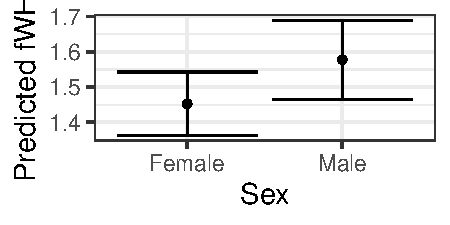
\includegraphics{bookdown-demo_files/figure-latex/unnamed-chunk-14-1.pdf}

\hypertarget{diy-method}{%
\section{DIY Method}\label{diy-method}}

\hypertarget{creating-a-hypothetical-dataset}{%
\subsection{Creating a hypothetical dataset}\label{creating-a-hypothetical-dataset}}

We would like to create a hypothetical dataset where one predictor variable varies, and all the rest stay fixed. Let's choose \texttt{AssR}. We use \texttt{expand.grid()}:

\begin{Shaded}
\begin{Highlighting}[]
\NormalTok{fake_data <-}\StringTok{ }\KeywordTok{expand.grid}\NormalTok{(}\DataTypeTok{AssR =} \KeywordTok{seq}\NormalTok{(}\DataTypeTok{from=}\FloatTok{1.8}\NormalTok{, }\DataTypeTok{to=}\FloatTok{5.7}\NormalTok{, }\DataTypeTok{by=}\FloatTok{0.05}\NormalTok{),}
                         \DataTypeTok{weight =} \DecValTok{40}\NormalTok{,}
                         \DataTypeTok{Sex =} \StringTok{'Female'}\NormalTok{,}
                         \DataTypeTok{Group =} \StringTok{'Twycross'}\NormalTok{)}
\KeywordTok{glimpse}\NormalTok{(fake_data)}
\end{Highlighting}
\end{Shaded}

\begin{verbatim}
## Observations: 79
## Variables: 4
## $ AssR   <dbl> 1.80, 1.85, 1.90, 1.95, 2.00, 2.05, 2.10, 2.15, 2.20, 2...
## $ weight <dbl> 40, 40, 40, 40, 40, 40, 40, 40, 40, 40, 40, 40, 40, 40,...
## $ Sex    <fct> Female, Female, Female, Female, Female, Female, Female,...
## $ Group  <fct> Twycross, Twycross, Twycross, Twycross, Twycross, Twycr...
\end{verbatim}

Now, make predictions for our fake data.

\begin{Shaded}
\begin{Highlighting}[]
\NormalTok{preds <-}\StringTok{ }\KeywordTok{predict}\NormalTok{(mlr3, }\DataTypeTok{newdata =}\NormalTok{ fake_data, }\DataTypeTok{se.fit =} \OtherTok{TRUE}\NormalTok{)}
\NormalTok{fake_data <-}\StringTok{ }\NormalTok{fake_data }\OperatorTok
\StringTok{  }\KeywordTok{mutate}\NormalTok{(}\DataTypeTok{fitted =}\NormalTok{ preds}\OperatorTok{$}\NormalTok{fit,}
         \DataTypeTok{se.fit =}\NormalTok{ preds}\OperatorTok{$}\NormalTok{se.fit)}
\KeywordTok{glimpse}\NormalTok{(fake_data)}
\end{Highlighting}
\end{Shaded}

\begin{verbatim}
## Observations: 79
## Variables: 6
## $ AssR   <dbl> 1.80, 1.85, 1.90, 1.95, 2.00, 2.05, 2.10, 2.15, 2.20, 2...
## $ weight <dbl> 40, 40, 40, 40, 40, 40, 40, 40, 40, 40, 40, 40, 40, 40,...
## $ Sex    <fct> Female, Female, Female, Female, Female, Female, Female,...
## $ Group  <fct> Twycross, Twycross, Twycross, Twycross, Twycross, Twycr...
## $ fitted <dbl> 1.149038, 1.152256, 1.155474, 1.158692, 1.161910, 1.165...
## $ se.fit <dbl> 0.08347207, 0.08267088, 0.08187552, 0.08108616, 0.08030...
\end{verbatim}

How do we go from \emph{standard errors} to \emph{confidence intervals}? We can either do this before plotting, or while plotting. To do it before and add the results to the hypothetical dataset:

\begin{Shaded}
\begin{Highlighting}[]
\NormalTok{fake_data <-}\StringTok{ }\NormalTok{fake_data }\OperatorTok
\StringTok{  }\KeywordTok{mutate}\NormalTok{(}\DataTypeTok{CI_lower =}\NormalTok{ fitted }\OperatorTok{-}\StringTok{ }\FloatTok{1.96}\OperatorTok{*}\NormalTok{se.fit,}
         \DataTypeTok{CI_upper =}\NormalTok{ fitted }\OperatorTok{+}\StringTok{ }\FloatTok{1.96}\OperatorTok{*}\NormalTok{se.fit)}
\KeywordTok{glimpse}\NormalTok{(fake_data)}
\end{Highlighting}
\end{Shaded}

\begin{verbatim}
## Observations: 79
## Variables: 8
## $ AssR     <dbl> 1.80, 1.85, 1.90, 1.95, 2.00, 2.05, 2.10, 2.15, 2.20,...
## $ weight   <dbl> 40, 40, 40, 40, 40, 40, 40, 40, 40, 40, 40, 40, 40, 4...
## $ Sex      <fct> Female, Female, Female, Female, Female, Female, Femal...
## $ Group    <fct> Twycross, Twycross, Twycross, Twycross, Twycross, Twy...
## $ fitted   <dbl> 1.149038, 1.152256, 1.155474, 1.158692, 1.161910, 1.1...
## $ se.fit   <dbl> 0.08347207, 0.08267088, 0.08187552, 0.08108616, 0.080...
## $ CI_lower <dbl> 0.9854326, 0.9902210, 0.9949980, 0.9997632, 1.0045164...
## $ CI_upper <dbl> 1.312643, 1.314291, 1.315950, 1.317621, 1.319304, 1.3...
\end{verbatim}

\hypertarget{making-the-plot}{%
\subsection{Making the plot}\label{making-the-plot}}

Now, we just need to plot!

\begin{Shaded}
\begin{Highlighting}[]
\KeywordTok{gf_line}\NormalTok{(fitted }\OperatorTok{~}\StringTok{ }\NormalTok{AssR, }\DataTypeTok{data=}\NormalTok{fake_data) }\OperatorTok\StringTok{ }
\StringTok{  }\KeywordTok{gf_labs}\NormalTok{(}\DataTypeTok{y=}\StringTok{'Predicted}\CharTok{\textbackslash{}n}\StringTok{fWHR'}\NormalTok{) }\OperatorTok
\StringTok{  }\KeywordTok{gf_ribbon}\NormalTok{(CI_lower }\OperatorTok{+}\StringTok{ }\NormalTok{CI_upper }\OperatorTok{~}\StringTok{ }\NormalTok{AssR, }\DataTypeTok{data =}\NormalTok{ fake_data)}
\end{Highlighting}
\end{Shaded}

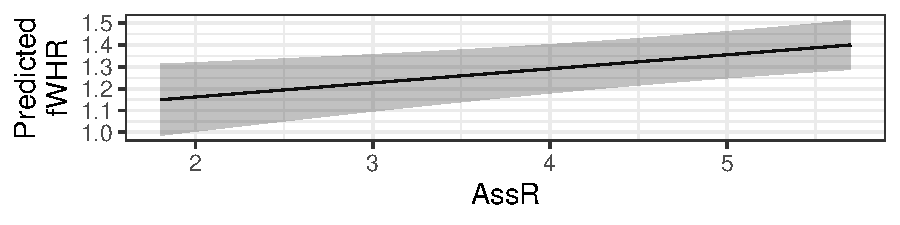
\includegraphics{bookdown-demo_files/figure-latex/unnamed-chunk-18-1.pdf}

If we wanted to figure out the CI bounds \emph{while} plotting, we could calculate them on the fly like this:

\begin{Shaded}
\begin{Highlighting}[]
\KeywordTok{gf_line}\NormalTok{(fitted }\OperatorTok{~}\StringTok{ }\NormalTok{AssR, }\DataTypeTok{data=}\NormalTok{fake_data) }\OperatorTok\StringTok{ }
\StringTok{  }\KeywordTok{gf_labs}\NormalTok{(}\DataTypeTok{y=}\StringTok{'Predicted}\CharTok{\textbackslash{}n}\StringTok{fWHR'}\NormalTok{) }\OperatorTok
\StringTok{  }\KeywordTok{gf_ribbon}\NormalTok{((fitted }\OperatorTok{-}\StringTok{ }\FloatTok{1.96}\OperatorTok{*}\NormalTok{se.fit ) }\OperatorTok{+}\StringTok{ }\NormalTok{(fitted }\OperatorTok{+}\StringTok{ }\FloatTok{1.96}\OperatorTok{*}\NormalTok{se.fit) }\OperatorTok{~}\StringTok{ }\NormalTok{AssR,}
            \DataTypeTok{data =}\NormalTok{ fake_data)}
\end{Highlighting}
\end{Shaded}

(which will look just the same).

\hypertarget{categorical-predictors}{%
\subsection{Categorical predictors}\label{categorical-predictors}}

What will be different if the predictor of interest is \emph{categorical}?

\begin{itemize}
\item
  hypothetical data:
\item
  plot:
\end{itemize}

\begin{Shaded}
\begin{Highlighting}[]
\NormalTok{fake_sex_data <-}\StringTok{ }\KeywordTok{expand.grid}\NormalTok{(}\DataTypeTok{AssR =} \FloatTok{4.51}\NormalTok{,}
                         \DataTypeTok{weight =} \DecValTok{40}\NormalTok{,}
                         \DataTypeTok{Sex =} \KeywordTok{c}\NormalTok{(}\StringTok{'Male'}\NormalTok{, }\StringTok{'Female'}\NormalTok{),}
                         \DataTypeTok{Group =} \StringTok{'Twycross'}\NormalTok{)}
\NormalTok{preds <-}\StringTok{ }\KeywordTok{predict}\NormalTok{(mlr3, }\DataTypeTok{newdata =}\NormalTok{ fake_sex_data, }\DataTypeTok{se.fit =} \OtherTok{TRUE}\NormalTok{)}
\NormalTok{fake_sex_data <-}\StringTok{ }\NormalTok{fake_sex_data }\OperatorTok
\StringTok{  }\KeywordTok{mutate}\NormalTok{(}\DataTypeTok{fitted =}\NormalTok{ preds}\OperatorTok{$}\NormalTok{fit,}
         \DataTypeTok{se.fit =}\NormalTok{ preds}\OperatorTok{$}\NormalTok{se.fit)}
\KeywordTok{gf_point}\NormalTok{(fitted }\OperatorTok{~}\StringTok{ }\NormalTok{Sex, }\DataTypeTok{data=}\NormalTok{fake_sex_data) }\OperatorTok\StringTok{ }
\StringTok{  }\KeywordTok{gf_labs}\NormalTok{(}\DataTypeTok{y=}\StringTok{'Predicted fWHR'}\NormalTok{) }\OperatorTok
\StringTok{  }\KeywordTok{gf_errorbar}\NormalTok{((fitted }\OperatorTok{-}\StringTok{ }\FloatTok{1.96}\OperatorTok{*}\NormalTok{se.fit ) }\OperatorTok{+}\StringTok{ }\NormalTok{(fitted }\OperatorTok{+}\StringTok{ }\FloatTok{1.96}\OperatorTok{*}\NormalTok{se.fit) }\OperatorTok{~}\StringTok{ }\NormalTok{Sex, }
            \DataTypeTok{data =}\NormalTok{ fake_sex_data)}
\end{Highlighting}
\end{Shaded}

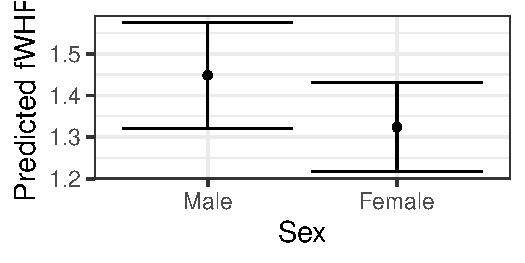
\includegraphics{bookdown-demo_files/figure-latex/unnamed-chunk-20-1.pdf}

\hypertarget{model-selection-using-information-criteria}{%
\chapter{Model Selection Using Information Criteria}\label{model-selection-using-information-criteria}}

So far, we have learned to fit models with multiple predictors, both quantitative and categorical, and to assess whether required conditions are met for linear regression to be an appropriate model for a dataset.

One missing piece is: If I have an appropriate model with a set of multiple predictors, how can I choose which predictors are worth retaining in a ``best'' model for the data (and which ones have no relationship, or a weak relationship, with the response, so should be discarded)?

\hypertarget{data-and-model}{%
\section{Data and Model}\label{data-and-model}}

Today we will recreate part of the analysis from \href{https://doi.org/10.1111/1365-2664.12798}{\emph{Vertebrate community composition and diversity declines along a defaunation gradient radiating from rural villages in Gabon}}, by Sally Koerner and colleagues. They investigated the relationship between rural villages, hunting, and wildlife in Gabon. They asked how monkey abundance depends on distance from villages, village size, and vegetation characteristics. They shared their data at \href{https://datadryad.org/stash/dataset/doi:10.5061/dryad.vs97g}{Dryad.org} and we can read it in and fit a regression model like this:

\begin{Shaded}
\begin{Highlighting}[]
\NormalTok{defaun <-}\StringTok{ }\KeywordTok{read.csv}\NormalTok{(}\StringTok{'http://sldr.netlify.com/data/koerner_gabon_defaunation.csv'}\NormalTok{)}
\end{Highlighting}
\end{Shaded}

\begin{Shaded}
\begin{Highlighting}[]
\NormalTok{ape_mod <-}\StringTok{ }\KeywordTok{lm}\NormalTok{(RA_Apes }\OperatorTok{~}\StringTok{ }\NormalTok{Veg_DBH }\OperatorTok{+}\StringTok{ }\NormalTok{Veg_Canopy }\OperatorTok{+}\StringTok{ }\NormalTok{Veg_Understory }\OperatorTok{+}
\StringTok{                   }\NormalTok{Veg_Rich }\OperatorTok{+}\StringTok{ }\NormalTok{Veg_Stems }\OperatorTok{+}\StringTok{ }\NormalTok{Veg_liana }\OperatorTok{+}
\StringTok{                   }\NormalTok{LandUse }\OperatorTok{+}\StringTok{ }\NormalTok{Distance }\OperatorTok{+}\StringTok{ }\NormalTok{NumHouseholds, }\DataTypeTok{data =}\NormalTok{ defaun)}
\KeywordTok{summary}\NormalTok{(ape_mod)}
\end{Highlighting}
\end{Shaded}

\begin{verbatim}
## 
## Call:
## lm(formula = RA_Apes ~ Veg_DBH + Veg_Canopy + Veg_Understory + 
##     Veg_Rich + Veg_Stems + Veg_liana + LandUse + Distance + NumHouseholds, 
##     data = defaun)
## 
## Residuals:
##     Min      1Q  Median      3Q     Max 
## -3.9857 -0.9419 -0.0360  0.8239  6.3832 
## 
## Coefficients:
##                 Estimate Std. Error t value Pr(>|t|)  
## (Intercept)     5.752517  13.372210   0.430   0.6741  
## Veg_DBH        -0.093171   0.073114  -1.274   0.2249  
## Veg_Canopy      0.670094   2.062545   0.325   0.7504  
## Veg_Understory -1.691235   2.071299  -0.817   0.4289  
## Veg_Rich        0.361960   0.480362   0.754   0.4646  
## Veg_Stems      -0.097211   0.169073  -0.575   0.5751  
## Veg_liana      -0.158505   0.253031  -0.626   0.5419  
## LandUseNeither  1.696755   2.058937   0.824   0.4247  
## LandUsePark    -2.947189   2.222710  -1.326   0.2077  
## Distance        0.302626   0.119865   2.525   0.0254 *
## NumHouseholds  -0.002107   0.043458  -0.048   0.9621  
## ---
## Signif. codes:  0 '***' 0.001 '**' 0.01 '*' 0.05 '.' 0.1 ' ' 1
## 
## Residual standard error: 2.725 on 13 degrees of freedom
## Multiple R-squared:  0.5439, Adjusted R-squared:  0.1931 
## F-statistic: 1.551 on 10 and 13 DF,  p-value: 0.2262
\end{verbatim}

\begin{Shaded}
\begin{Highlighting}[]
\KeywordTok{as.numeric}\NormalTok{(}\KeywordTok{logLik}\NormalTok{(ape_mod))}
\end{Highlighting}
\end{Shaded}

\begin{verbatim}
## [1] -50.75799
\end{verbatim}

\hypertarget{calculations}{%
\section{Calculations}\label{calculations}}

\begin{itemize}
\item
  Information criteria allow us to \textbf{balance the conflicting goals} of having a model that \emph{fits the data as well as possible} (which pushes us toward models with more predictors) and \emph{parsimony} (choosing the simplest model, with the fewest predictors, that works for the data and research question). The basic idea is that we \textbf{minimize} the quantity \(-(2LogLikelihood - penalty) = -2LogLikelihood + penalty\)
\item
  AIC is computed according to \(-2LogLikelihood +2k\), where \(k\) is the number of coefficients being estimated (don't forget \(\sigma\)!) \textbf{Smaller AIC is better.}
\item
  BIC is computed according to \(-2LogLikelihood + ln(n)k\), where \(n\) is the number of observations (rows) in the dataset and \(k\) is the number of coefficients being estimated. \textbf{Smaller BIC is better.}
\item
  Verify that the BIC for this model is 139.65.
\end{itemize}

\hypertarget{decisions-with-ics}{%
\section{Decisions with ICs}\label{decisions-with-ics}}

The following rules of thumb (\textbf{not} laws, just common rules of thumb) may help you make decisions with ICs:

\begin{itemize}
\tightlist
\item
  A model with lower IC \emph{by at least 3 units} is notably better.
\item
  If two or more models have ICs \emph{within} 3 IC units of each other, there is not a lot of difference between them. Here, we usually choose the model with fewest predictors.
\item
  In some cases, if the research question is to measure the influence of some particular predictor on the response, but \emph{the IC does not strongly support including that predictor} in the best model (IC difference less than 3), you might want to keep it in anyway and then discuss the situation honestly, for example, ``AIC does not provide strong support for including predictor x in the best model, but the model including predictor x indicates that as x increases the response decreases slightly. More research would be needed\ldots{}''
\end{itemize}

\hypertarget{all-possible-subsets-selection}{%
\section{All-possible-subsets Selection}\label{all-possible-subsets-selection}}

The model we just fitted is our \emph{full model}, with all predictors of potential interest included. How can we use information criteria to choose the best model from possible models with subsets of the predictors?

We can use the \texttt{dredge()} function from the \texttt{MuMIn} package to get and display ICs for all these models.

Before using dredge, we need to make sure our dataset has no missing values, and also set the ``na.action'' input for our model (can be done in call to \texttt{lm(...,\ na.action\ =\ \textquotesingle{}na.fail\textquotesingle{})} also).

\begin{Shaded}
\begin{Highlighting}[]
\KeywordTok{require}\NormalTok{(MuMIn)}
\NormalTok{ape_mod <-}\StringTok{ }\NormalTok{ape_mod }\OperatorTok\StringTok{ }\KeywordTok{update}\NormalTok{(}\DataTypeTok{na.action =} \StringTok{'na.fail'}\NormalTok{)}
\NormalTok{ape_dredge <-}\StringTok{ }\KeywordTok{dredge}\NormalTok{(ape_mod, }\DataTypeTok{rank=}\StringTok{'BIC'}\NormalTok{)}
\end{Highlighting}
\end{Shaded}

\begin{verbatim}
## Fixed term is "(Intercept)"
\end{verbatim}

\begin{Shaded}
\begin{Highlighting}[]
\NormalTok{pander}\OperatorTok{::}\KeywordTok{pander}\NormalTok{(}\KeywordTok{head}\NormalTok{(ape_dredge, }\DecValTok{7}\NormalTok{))}
\end{Highlighting}
\end{Shaded}

\begin{longtable}[]{@{}cccccc@{}}
\caption{Table continues below}\tabularnewline
\toprule
\begin{minipage}[b]{0.11\columnwidth}\centering
~\strut
\end{minipage} & \begin{minipage}[b]{0.16\columnwidth}\centering
(Intercept)\strut
\end{minipage} & \begin{minipage}[b]{0.12\columnwidth}\centering
Distance\strut
\end{minipage} & \begin{minipage}[b]{0.11\columnwidth}\centering
LandUse\strut
\end{minipage} & \begin{minipage}[b]{0.18\columnwidth}\centering
NumHouseholds\strut
\end{minipage} & \begin{minipage}[b]{0.15\columnwidth}\centering
Veg\_Canopy\strut
\end{minipage}\tabularnewline
\midrule
\endfirsthead
\toprule
\begin{minipage}[b]{0.11\columnwidth}\centering
~\strut
\end{minipage} & \begin{minipage}[b]{0.16\columnwidth}\centering
(Intercept)\strut
\end{minipage} & \begin{minipage}[b]{0.12\columnwidth}\centering
Distance\strut
\end{minipage} & \begin{minipage}[b]{0.11\columnwidth}\centering
LandUse\strut
\end{minipage} & \begin{minipage}[b]{0.18\columnwidth}\centering
NumHouseholds\strut
\end{minipage} & \begin{minipage}[b]{0.15\columnwidth}\centering
Veg\_Canopy\strut
\end{minipage}\tabularnewline
\midrule
\endhead
\begin{minipage}[t]{0.11\columnwidth}\centering
\textbf{258}\strut
\end{minipage} & \begin{minipage}[t]{0.16\columnwidth}\centering
8.753\strut
\end{minipage} & \begin{minipage}[t]{0.12\columnwidth}\centering
0.195\strut
\end{minipage} & \begin{minipage}[t]{0.11\columnwidth}\centering
NA\strut
\end{minipage} & \begin{minipage}[t]{0.18\columnwidth}\centering
NA\strut
\end{minipage} & \begin{minipage}[t]{0.15\columnwidth}\centering
NA\strut
\end{minipage}\tabularnewline
\begin{minipage}[t]{0.11\columnwidth}\centering
\textbf{2}\strut
\end{minipage} & \begin{minipage}[t]{0.16\columnwidth}\centering
-0.6912\strut
\end{minipage} & \begin{minipage}[t]{0.12\columnwidth}\centering
0.2303\strut
\end{minipage} & \begin{minipage}[t]{0.11\columnwidth}\centering
NA\strut
\end{minipage} & \begin{minipage}[t]{0.18\columnwidth}\centering
NA\strut
\end{minipage} & \begin{minipage}[t]{0.15\columnwidth}\centering
NA\strut
\end{minipage}\tabularnewline
\begin{minipage}[t]{0.11\columnwidth}\centering
\textbf{274}\strut
\end{minipage} & \begin{minipage}[t]{0.16\columnwidth}\centering
11.44\strut
\end{minipage} & \begin{minipage}[t]{0.12\columnwidth}\centering
0.1848\strut
\end{minipage} & \begin{minipage}[t]{0.11\columnwidth}\centering
NA\strut
\end{minipage} & \begin{minipage}[t]{0.18\columnwidth}\centering
NA\strut
\end{minipage} & \begin{minipage}[t]{0.15\columnwidth}\centering
NA\strut
\end{minipage}\tabularnewline
\begin{minipage}[t]{0.11\columnwidth}\centering
\textbf{322}\strut
\end{minipage} & \begin{minipage}[t]{0.16\columnwidth}\centering
11.9\strut
\end{minipage} & \begin{minipage}[t]{0.12\columnwidth}\centering
0.2033\strut
\end{minipage} & \begin{minipage}[t]{0.11\columnwidth}\centering
NA\strut
\end{minipage} & \begin{minipage}[t]{0.18\columnwidth}\centering
NA\strut
\end{minipage} & \begin{minipage}[t]{0.15\columnwidth}\centering
NA\strut
\end{minipage}\tabularnewline
\begin{minipage}[t]{0.11\columnwidth}\centering
\textbf{290}\strut
\end{minipage} & \begin{minipage}[t]{0.16\columnwidth}\centering
9.805\strut
\end{minipage} & \begin{minipage}[t]{0.12\columnwidth}\centering
0.1884\strut
\end{minipage} & \begin{minipage}[t]{0.11\columnwidth}\centering
NA\strut
\end{minipage} & \begin{minipage}[t]{0.18\columnwidth}\centering
NA\strut
\end{minipage} & \begin{minipage}[t]{0.15\columnwidth}\centering
NA\strut
\end{minipage}\tabularnewline
\begin{minipage}[t]{0.11\columnwidth}\centering
\textbf{386}\strut
\end{minipage} & \begin{minipage}[t]{0.16\columnwidth}\centering
9.49\strut
\end{minipage} & \begin{minipage}[t]{0.12\columnwidth}\centering
0.1976\strut
\end{minipage} & \begin{minipage}[t]{0.11\columnwidth}\centering
NA\strut
\end{minipage} & \begin{minipage}[t]{0.18\columnwidth}\centering
NA\strut
\end{minipage} & \begin{minipage}[t]{0.15\columnwidth}\centering
NA\strut
\end{minipage}\tabularnewline
\begin{minipage}[t]{0.11\columnwidth}\centering
\textbf{266}\strut
\end{minipage} & \begin{minipage}[t]{0.16\columnwidth}\centering
7.783\strut
\end{minipage} & \begin{minipage}[t]{0.12\columnwidth}\centering
0.1896\strut
\end{minipage} & \begin{minipage}[t]{0.11\columnwidth}\centering
NA\strut
\end{minipage} & \begin{minipage}[t]{0.18\columnwidth}\centering
NA\strut
\end{minipage} & \begin{minipage}[t]{0.15\columnwidth}\centering
0.2771\strut
\end{minipage}\tabularnewline
\bottomrule
\end{longtable}

\begin{longtable}[]{@{}ccccccc@{}}
\caption{Table continues below}\tabularnewline
\toprule
\begin{minipage}[b]{0.10\columnwidth}\centering
~\strut
\end{minipage} & \begin{minipage}[b]{0.11\columnwidth}\centering
Veg\_DBH\strut
\end{minipage} & \begin{minipage}[b]{0.12\columnwidth}\centering
Veg\_liana\strut
\end{minipage} & \begin{minipage}[b]{0.11\columnwidth}\centering
Veg\_Rich\strut
\end{minipage} & \begin{minipage}[b]{0.12\columnwidth}\centering
Veg\_Stems\strut
\end{minipage} & \begin{minipage}[b]{0.18\columnwidth}\centering
Veg\_Understory\strut
\end{minipage} & \begin{minipage}[b]{0.05\columnwidth}\centering
df\strut
\end{minipage}\tabularnewline
\midrule
\endfirsthead
\toprule
\begin{minipage}[b]{0.10\columnwidth}\centering
~\strut
\end{minipage} & \begin{minipage}[b]{0.11\columnwidth}\centering
Veg\_DBH\strut
\end{minipage} & \begin{minipage}[b]{0.12\columnwidth}\centering
Veg\_liana\strut
\end{minipage} & \begin{minipage}[b]{0.11\columnwidth}\centering
Veg\_Rich\strut
\end{minipage} & \begin{minipage}[b]{0.12\columnwidth}\centering
Veg\_Stems\strut
\end{minipage} & \begin{minipage}[b]{0.18\columnwidth}\centering
Veg\_Understory\strut
\end{minipage} & \begin{minipage}[b]{0.05\columnwidth}\centering
df\strut
\end{minipage}\tabularnewline
\midrule
\endhead
\begin{minipage}[t]{0.10\columnwidth}\centering
\textbf{258}\strut
\end{minipage} & \begin{minipage}[t]{0.11\columnwidth}\centering
NA\strut
\end{minipage} & \begin{minipage}[t]{0.12\columnwidth}\centering
NA\strut
\end{minipage} & \begin{minipage}[t]{0.11\columnwidth}\centering
NA\strut
\end{minipage} & \begin{minipage}[t]{0.12\columnwidth}\centering
NA\strut
\end{minipage} & \begin{minipage}[t]{0.18\columnwidth}\centering
-2.988\strut
\end{minipage} & \begin{minipage}[t]{0.05\columnwidth}\centering
4\strut
\end{minipage}\tabularnewline
\begin{minipage}[t]{0.10\columnwidth}\centering
\textbf{2}\strut
\end{minipage} & \begin{minipage}[t]{0.11\columnwidth}\centering
NA\strut
\end{minipage} & \begin{minipage}[t]{0.12\columnwidth}\centering
NA\strut
\end{minipage} & \begin{minipage}[t]{0.11\columnwidth}\centering
NA\strut
\end{minipage} & \begin{minipage}[t]{0.12\columnwidth}\centering
NA\strut
\end{minipage} & \begin{minipage}[t]{0.18\columnwidth}\centering
NA\strut
\end{minipage} & \begin{minipage}[t]{0.05\columnwidth}\centering
3\strut
\end{minipage}\tabularnewline
\begin{minipage}[t]{0.10\columnwidth}\centering
\textbf{274}\strut
\end{minipage} & \begin{minipage}[t]{0.11\columnwidth}\centering
-0.04551\strut
\end{minipage} & \begin{minipage}[t]{0.12\columnwidth}\centering
NA\strut
\end{minipage} & \begin{minipage}[t]{0.11\columnwidth}\centering
NA\strut
\end{minipage} & \begin{minipage}[t]{0.12\columnwidth}\centering
NA\strut
\end{minipage} & \begin{minipage}[t]{0.18\columnwidth}\centering
-3.144\strut
\end{minipage} & \begin{minipage}[t]{0.05\columnwidth}\centering
5\strut
\end{minipage}\tabularnewline
\begin{minipage}[t]{0.10\columnwidth}\centering
\textbf{322}\strut
\end{minipage} & \begin{minipage}[t]{0.11\columnwidth}\centering
NA\strut
\end{minipage} & \begin{minipage}[t]{0.12\columnwidth}\centering
NA\strut
\end{minipage} & \begin{minipage}[t]{0.11\columnwidth}\centering
-0.1939\strut
\end{minipage} & \begin{minipage}[t]{0.12\columnwidth}\centering
NA\strut
\end{minipage} & \begin{minipage}[t]{0.18\columnwidth}\centering
-3.11\strut
\end{minipage} & \begin{minipage}[t]{0.05\columnwidth}\centering
5\strut
\end{minipage}\tabularnewline
\begin{minipage}[t]{0.10\columnwidth}\centering
\textbf{290}\strut
\end{minipage} & \begin{minipage}[t]{0.11\columnwidth}\centering
NA\strut
\end{minipage} & \begin{minipage}[t]{0.12\columnwidth}\centering
-0.09802\strut
\end{minipage} & \begin{minipage}[t]{0.11\columnwidth}\centering
NA\strut
\end{minipage} & \begin{minipage}[t]{0.12\columnwidth}\centering
NA\strut
\end{minipage} & \begin{minipage}[t]{0.18\columnwidth}\centering
-2.952\strut
\end{minipage} & \begin{minipage}[t]{0.05\columnwidth}\centering
5\strut
\end{minipage}\tabularnewline
\begin{minipage}[t]{0.10\columnwidth}\centering
\textbf{386}\strut
\end{minipage} & \begin{minipage}[t]{0.11\columnwidth}\centering
NA\strut
\end{minipage} & \begin{minipage}[t]{0.12\columnwidth}\centering
NA\strut
\end{minipage} & \begin{minipage}[t]{0.11\columnwidth}\centering
NA\strut
\end{minipage} & \begin{minipage}[t]{0.12\columnwidth}\centering
-0.03113\strut
\end{minipage} & \begin{minipage}[t]{0.18\columnwidth}\centering
-2.904\strut
\end{minipage} & \begin{minipage}[t]{0.05\columnwidth}\centering
5\strut
\end{minipage}\tabularnewline
\begin{minipage}[t]{0.10\columnwidth}\centering
\textbf{266}\strut
\end{minipage} & \begin{minipage}[t]{0.11\columnwidth}\centering
NA\strut
\end{minipage} & \begin{minipage}[t]{0.12\columnwidth}\centering
NA\strut
\end{minipage} & \begin{minipage}[t]{0.11\columnwidth}\centering
NA\strut
\end{minipage} & \begin{minipage}[t]{0.12\columnwidth}\centering
NA\strut
\end{minipage} & \begin{minipage}[t]{0.18\columnwidth}\centering
-2.964\strut
\end{minipage} & \begin{minipage}[t]{0.05\columnwidth}\centering
5\strut
\end{minipage}\tabularnewline
\bottomrule
\end{longtable}

\begin{longtable}[]{@{}ccccc@{}}
\toprule
\begin{minipage}[b]{0.12\columnwidth}\centering
~\strut
\end{minipage} & \begin{minipage}[b]{0.11\columnwidth}\centering
logLik\strut
\end{minipage} & \begin{minipage}[b]{0.10\columnwidth}\centering
BIC\strut
\end{minipage} & \begin{minipage}[b]{0.11\columnwidth}\centering
delta\strut
\end{minipage} & \begin{minipage}[b]{0.12\columnwidth}\centering
weight\strut
\end{minipage}\tabularnewline
\midrule
\endhead
\begin{minipage}[t]{0.12\columnwidth}\centering
\textbf{258}\strut
\end{minipage} & \begin{minipage}[t]{0.11\columnwidth}\centering
-53.9\strut
\end{minipage} & \begin{minipage}[t]{0.10\columnwidth}\centering
120.5\strut
\end{minipage} & \begin{minipage}[t]{0.11\columnwidth}\centering
0\strut
\end{minipage} & \begin{minipage}[t]{0.12\columnwidth}\centering
0.3284\strut
\end{minipage}\tabularnewline
\begin{minipage}[t]{0.12\columnwidth}\centering
\textbf{2}\strut
\end{minipage} & \begin{minipage}[t]{0.11\columnwidth}\centering
-55.8\strut
\end{minipage} & \begin{minipage}[t]{0.10\columnwidth}\centering
121.1\strut
\end{minipage} & \begin{minipage}[t]{0.11\columnwidth}\centering
0.6241\strut
\end{minipage} & \begin{minipage}[t]{0.12\columnwidth}\centering
0.2404\strut
\end{minipage}\tabularnewline
\begin{minipage}[t]{0.12\columnwidth}\centering
\textbf{274}\strut
\end{minipage} & \begin{minipage}[t]{0.11\columnwidth}\centering
-53.38\strut
\end{minipage} & \begin{minipage}[t]{0.10\columnwidth}\centering
122.7\strut
\end{minipage} & \begin{minipage}[t]{0.11\columnwidth}\centering
2.146\strut
\end{minipage} & \begin{minipage}[t]{0.12\columnwidth}\centering
0.1123\strut
\end{minipage}\tabularnewline
\begin{minipage}[t]{0.12\columnwidth}\centering
\textbf{322}\strut
\end{minipage} & \begin{minipage}[t]{0.11\columnwidth}\centering
-53.55\strut
\end{minipage} & \begin{minipage}[t]{0.10\columnwidth}\centering
123\strut
\end{minipage} & \begin{minipage}[t]{0.11\columnwidth}\centering
2.491\strut
\end{minipage} & \begin{minipage}[t]{0.12\columnwidth}\centering
0.09449\strut
\end{minipage}\tabularnewline
\begin{minipage}[t]{0.12\columnwidth}\centering
\textbf{290}\strut
\end{minipage} & \begin{minipage}[t]{0.11\columnwidth}\centering
-53.67\strut
\end{minipage} & \begin{minipage}[t]{0.10\columnwidth}\centering
123.2\strut
\end{minipage} & \begin{minipage}[t]{0.11\columnwidth}\centering
2.727\strut
\end{minipage} & \begin{minipage}[t]{0.12\columnwidth}\centering
0.08399\strut
\end{minipage}\tabularnewline
\begin{minipage}[t]{0.12\columnwidth}\centering
\textbf{386}\strut
\end{minipage} & \begin{minipage}[t]{0.11\columnwidth}\centering
-53.82\strut
\end{minipage} & \begin{minipage}[t]{0.10\columnwidth}\centering
123.5\strut
\end{minipage} & \begin{minipage}[t]{0.11\columnwidth}\centering
3.03\strut
\end{minipage} & \begin{minipage}[t]{0.12\columnwidth}\centering
0.0722\strut
\end{minipage}\tabularnewline
\begin{minipage}[t]{0.12\columnwidth}\centering
\textbf{266}\strut
\end{minipage} & \begin{minipage}[t]{0.11\columnwidth}\centering
-53.88\strut
\end{minipage} & \begin{minipage}[t]{0.10\columnwidth}\centering
123.7\strut
\end{minipage} & \begin{minipage}[t]{0.11\columnwidth}\centering
3.144\strut
\end{minipage} & \begin{minipage}[t]{0.12\columnwidth}\centering
0.0682\strut
\end{minipage}\tabularnewline
\bottomrule
\end{longtable}

\begin{itemize}
\tightlist
\item
  What is the best model according to BIC, for this dataset?
\end{itemize}

\hypertarget{which-ic-should-i-use}{%
\section{Which IC should I use?}\label{which-ic-should-i-use}}

AIC and BIC may give different best models, especially if the dataset is large. You may want to just choose one to use \emph{a priori} (before making calculations). You might prefer BIC if you want to err on the ``conservative'' side, as it is more likely to select a ``smaller'' model with fewer predictors. This is because of its larger penalty.

\hypertarget{quantities-derived-from-aic}{%
\section{Quantities derived from AIC}\label{quantities-derived-from-aic}}

\begin{itemize}
\tightlist
\item
  \(\Delta AIC\) is the AIC for a given model, minus the AIC of the best one in the dataset. (Same for \(\Delta BIC\))
\item
  \emph{Akaike weights} are values (ranging from 0-1) that measure the weight of evidence suggesting that a model is the best one (given that there is one best one in the set)
\end{itemize}

\hypertarget{important-caution}{%
\section{Important Caution}\label{important-caution}}

\textbf{Very important}: IC can \textbf{ONLY} be compared for models with the same response variable, and the exact same rows of data.

\hypertarget{likelihood}{%
\chapter{Likelihood}\label{likelihood}}

In the last section, we said that ``likelihood'' is a measure of goodness-of-fit of a model to a dataset. But what is it \emph{exactly} and just how do we compute it?

\hypertarget{data-1}{%
\section{Data}\label{data-1}}

Today's dataset was collected in Senegal in 2015-2016 in a survey carried out by UNICEF, of 5440 households in the urban area of Dakar, Senegal. Among these households, information was collected about 4453 children under 5 years old, including their \textbf{weights in kilograms.}

\begin{Shaded}
\begin{Highlighting}[]
\KeywordTok{gf_dhistogram}\NormalTok{(}\OperatorTok{~}\NormalTok{AN3, }\DataTypeTok{data=}\NormalTok{wt, }\DataTypeTok{binwidth=}\DecValTok{1}\NormalTok{) }\OperatorTok
\StringTok{  }\KeywordTok{gf_labs}\NormalTok{(}\DataTypeTok{x=}\StringTok{'Weight (kg)'}\NormalTok{, }\DataTypeTok{y=}\StringTok{'Probability}\CharTok{\textbackslash{}n}\StringTok{Density'}\NormalTok{) }\OperatorTok
\StringTok{  }\KeywordTok{gf_fitdistr}\NormalTok{(}\DataTypeTok{dist=}\StringTok{'dnorm'}\NormalTok{, }\DataTypeTok{size=}\FloatTok{1.3}\NormalTok{) }\OperatorTok
\StringTok{  }\KeywordTok{gf_refine}\NormalTok{(}\KeywordTok{scale_x_continuous}\NormalTok{(}\DataTypeTok{breaks=}\KeywordTok{seq}\NormalTok{(}\DataTypeTok{from=}\DecValTok{0}\NormalTok{, }\DataTypeTok{to=}\DecValTok{30}\NormalTok{, }\DataTypeTok{by=}\DecValTok{2}\NormalTok{)))}
\end{Highlighting}
\end{Shaded}

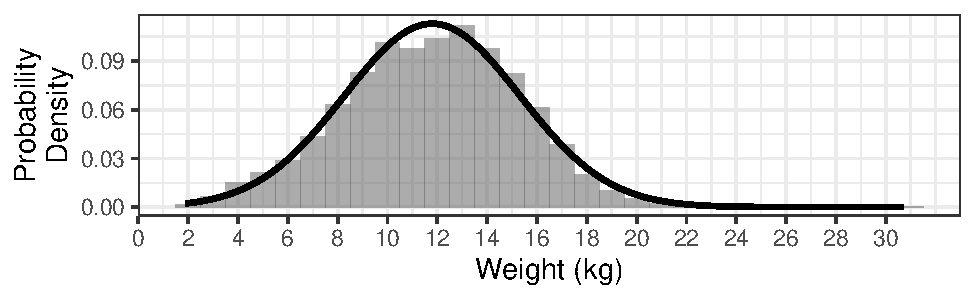
\includegraphics{bookdown-demo_files/figure-latex/unnamed-chunk-23-1.pdf}

\hypertarget{review---the-normal-probability-density-function-pdf}{%
\section{Review - the Normal probability density function (PDF)}\label{review---the-normal-probability-density-function-pdf}}

\[ f(x) = \frac{1}{\sqrt{2\pi\sigma^2}} e^{-\frac{(x-\mu)^2}{2\sigma^2}} \]

\hypertarget{a-simple-model}{%
\section{A simple model}\label{a-simple-model}}

The distribution of weights looks quite unimodal and symmetric, so we will model it with a normal distribution with mean 11.8 and standard deviation 3.53 (N( \(\mu=\) 11.8, \(\sigma=\) 3.53), black line).

\hypertarget{using-the-model-to-make-predictions}{%
\section{Using the Model to Make Predictions}\label{using-the-model-to-make-predictions}}

If you had to predict the weight of one child from this population, what weight would you guess?
\vspace{0.05in}

Is it more likely for a child in Dakar to weigh 10kg, or 20kg? How much more likely?

What is the \emph{probability} of a child in Dakar weighing 11.5 kg?

\hypertarget{likelihood-to-the-rescue}{%
\section{Likelihood to the Rescue!}\label{likelihood-to-the-rescue}}

Which is more likely: three children who weigh 11, 8.2, and 13kg, or three who weigh 10, 12.5 and 15 kg?

How did you:

\begin{itemize}
\tightlist
\item
  Find the likelihood of each observation?
\end{itemize}

\begin{itemize}
\tightlist
\item
  Combine the likelihoods of a set of three observations?
\end{itemize}

What did you have to assume about the set of observations?

\hypertarget{how-does-this-relate-to-linear-regression}{%
\section{How does this relate to linear regression?}\label{how-does-this-relate-to-linear-regression}}

What if we think of this situation as a linear regression problem (with no predictors)?

\begin{Shaded}
\begin{Highlighting}[]
\NormalTok{lm_version <-}\StringTok{ }\KeywordTok{lm}\NormalTok{(AN3 }\OperatorTok{~}\StringTok{ }\DecValTok{1}\NormalTok{, }\DataTypeTok{data =}\NormalTok{ wt)}
\KeywordTok{summary}\NormalTok{(lm_version)}
\end{Highlighting}
\end{Shaded}

\begin{verbatim}
## 
## Call:
## lm(formula = AN3 ~ 1, data = wt)
## 
## Residuals:
## <Labelled double>: Poids de l'enfant (kilogrammes)
##     Min      1Q  Median      3Q     Max 
## -9.8964 -2.3964  0.1036  2.4036 18.9036 
## 
## Labels:
##  value            label
##   99.9 poids non mesuré
## 
## Coefficients:
##             Estimate Std. Error t value Pr(>|t|)    
## (Intercept) 11.79644    0.05435   217.1   <2e-16 ***
## ---
## Signif. codes:  0 '***' 0.001 '**' 0.01 '*' 0.05 '.' 0.1 ' ' 1
## 
## Residual standard error: 3.529 on 4216 degrees of freedom
##   (235 observations deleted due to missingness)
\end{verbatim}

\hypertarget{model-equation}{%
\subsection{Model Equation:}\label{model-equation}}

\hypertarget{likelihood-of-a-dataset-given-a-model}{%
\section{Likelihood of a dataset, given a model}\label{likelihood-of-a-dataset-given-a-model}}

Finally, now, we can understand what we were computing when we did

\begin{Shaded}
\begin{Highlighting}[]
\KeywordTok{logLik}\NormalTok{(lm_version)}
\end{Highlighting}
\end{Shaded}

\begin{verbatim}
## 'log Lik.' -11301.19 (df=2)
\end{verbatim}

For our chosen regression model, we know that the residuals should have a normal distribution with mean 0 and standard deviation \(\sigma\) (estimated Residual Standard Error from R \texttt{summary()} output).

For each data point in the dataset, for a given regression model, we can compute a model prediction.

We can subtract the prediction from the observed response-variable values to get the residuals.

We can compute the \textbf{likelihood} (\(L\)) of this set of residuals by finding the likelihood of each individual residual \(e_i\) in a \(N(0, \sigma)\) distribution.

To get the likelihood of the full dataset given the model, we use the fact that the residuals are independent (they better be, because that was one of the conditions of of linear regression model) -- we can multiply the likelihoods of all the individual residuals together to get the joint likelihood of the full set.

\emph{That} is the ``likelihood'' that is used in the AIC and BIC calculations we considered earlier.

\bibliography{book.bib,packages.bib}


\end{document}
